% !Mode:: "TeX:UTF-8"

\titlepage

\begin{frame}{说在前面}
	\linespread{1.5}
	  \begin{itemize}[<+-|alert@+>]
	    \item \ba{好好画图啊!}
	    \item \ba{好好复习积分的计算啊!}
	    \item \ba{微分方程和级数忘得差不多了吧,现在还不复习啊?}
% 	    \item 不记得自己哪周交作业
	  \end{itemize}
\end{frame}

% \begin{frame}{需要注意的问题}
% 	\linespread{1.5}
% 	  \begin{itemize}%[<+-|alert@+>]
% 	    \item L'Hospital法则
% 	    \begin{itemize}
% 	      \item \it 只能应用于“$\df{\bm{0}}{\bm{0}}$”
% 	      和“$\df{\bm{\infty}}{\bm{\infty}}$”型
% 	      \item \it 及时使用无穷小代换进行简化
% 	      \item \it 不正规的符号:\b 
% 	      $\xlongequal{\footnotesize\mbox{“L”}}$、
% 	      $\xlongrightarrow{\footnotesize\mbox{“L'Hospital法则”}}$、
% 	      $\df{\bm{0}}{\bm{0}}$、$\df{\bm{\infty}}{\bm{\infty}}$
% 	    \end{itemize}
% 	    \item Taylor公式
% 	    \begin{itemize}
% 	      \item \it Taylor多项式不包含余项
% 	      \item \it 合并同次幂的系数
% 	      \item \it 尽量按照幂次由低到高排列,最后写余项
% 	    \end{itemize}
% 	  \end{itemize}
% \end{frame}

\section{10.1 重积分的概念与性质}

\begin{frame}
	\linespread{1.5}
	\ba{1.设平面区域$D$由$x=0,y=0,x+y=\df14,x+y=1$所围成,
  $\small I_1=\iint_D[\ln(x+y)]^3\d\sigma,
  I_2=\iint_D(x+y)^3\d\sigma,
  I_3=\iint_D[\sin(x+y)]^3\d\sigma.$
  请画出区域$D$的图形,并给出$I_1,I_2,I_3$的大小次序。}
	
	\bigskip
	
	\small 解:\it
	由已知$\df14\leq x+y\leq 1$,此时
	$$\ln(x+y)\leq 0<\sin(x+y)<x+y,$$
	进而对任意$(x,y)\in D$,总有
	$$[\ln(x+y)]^3\leq 0<[\sin(x+y)]^3<(x+y)^3,$$
	于是由重积分的保号性可知$I_1<I_3<I_2$。\fin
\end{frame}

\begin{frame}
	\linespread{1.5}
	\ba{2.设平面区域$D$为$(x-2)^2+(y-1)^2\leq1$,试比较积分
	  $I_1=\ds\iint_D(x+y)^2\d\sigma$和$I_2=\ds\iint_D(x+y)^3\d\sigma$
	  的大小。}
	
	\bigskip
	
	\small 解:\it
	当$(x-2)^2+(y-1)^2\leq1$时,总有$x+y>1$,进而
	对任意$(x,y)\in D$,总有
	$$(x+y)^3>(x+y)^2,$$
	于是由重积分的保号性可知$I_1<I_2$。\fin
\end{frame}

\section{10.2 二重积分的计算}

\begin{frame}
	\linespread{1.5}
	\ba{1.交换以下二重积分的积分次序:
	
	(1)$\dint_0^{2a}\dint_{\sqrt{2ax-x^2}}^{\sqrt{2ax}}
	f(x,y)\d y\d x,\;(a>0)$	}

	\bigskip
	
	\begin{columns}
		\begin{column}{.45\textwidth}
			\begin{center}
				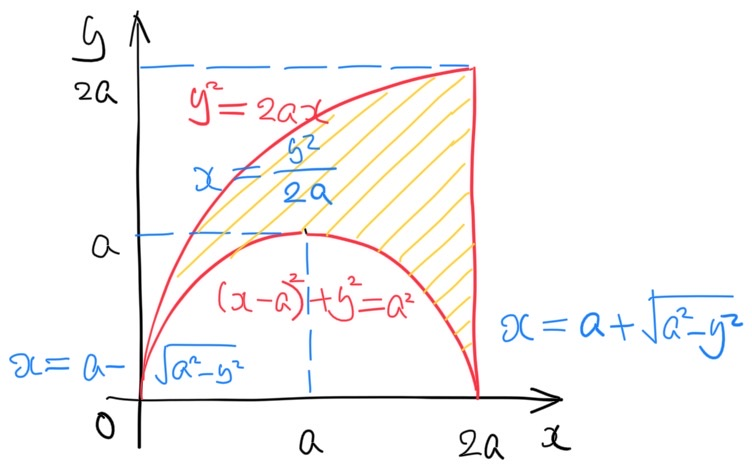
\includegraphics[width=\textwidth]{./images/ch10/10.2.1.1.jpg}
		% 		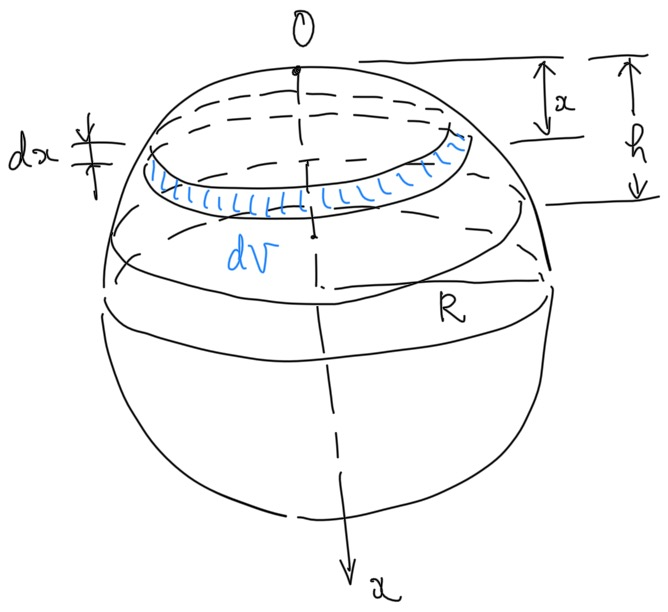
\includegraphics[width=6cm]{./images/ch6/topSp.jpg}
			\end{center}
		\end{column}
		\begin{column}{.55\textwidth}
			\small 解:\it
			如图,
			\begin{align*}
				\mbox{原式}=&\dint_0^{2a}\dint_{\frac{y^2}{2a}}^{2a}f(x,y)\d x\d y\\
				&-\dint_0^{a}\dint_{a-\sqrt{a^2-y^2}}^{a+\sqrt{a^2-y^2}}f(x,y)\d x\d y
			\end{align*}
		\end{column}
	\end{columns}
\end{frame}

\begin{frame}
	\linespread{1.5}
	\ba{(2)$\dint_0^1\dint_{1-y}^{1+y^2}f(x,y)\d x\d y$}

	\begin{center}
		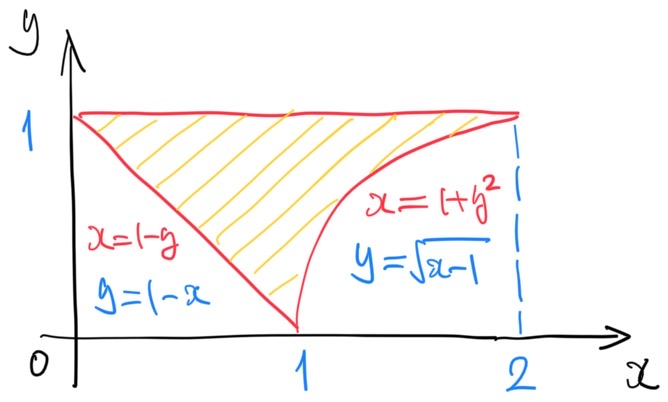
\includegraphics[width=0.45\textwidth]{./images/ch10/10.2.1.2.jpg}
% 		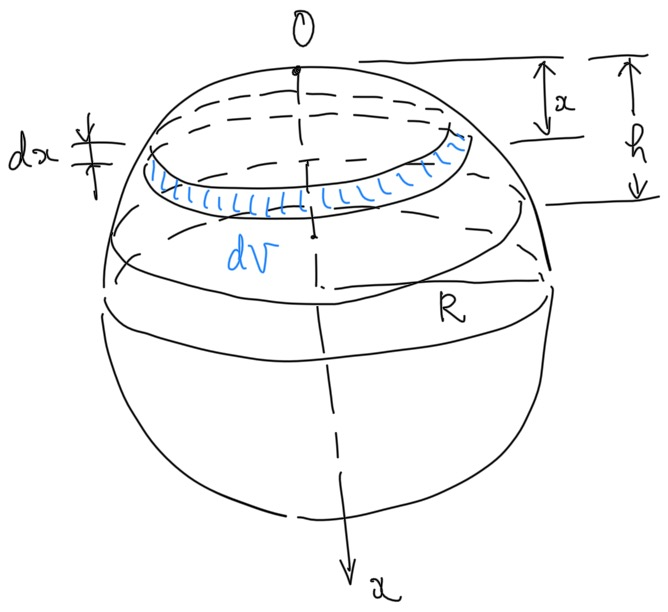
\includegraphics[width=6cm]{./images/ch6/topSp.jpg}
	\end{center}
	\small 解:\it
	如图,
	$$\mbox{原式}=\left(\dint_0^1\dint_{1-x}^1
	+\dint_1^2\dint_{\sqrt{x-1}}^1\right)
	f(x,y)\d y\d x$$
\end{frame}

\begin{frame}
	\linespread{1.5}
	\ba{(3)$\dint_0^{\pi}\dint_{-\sin\frac x2}^{\sin x}f(x,y)\d y\d x$}

	\begin{center}
		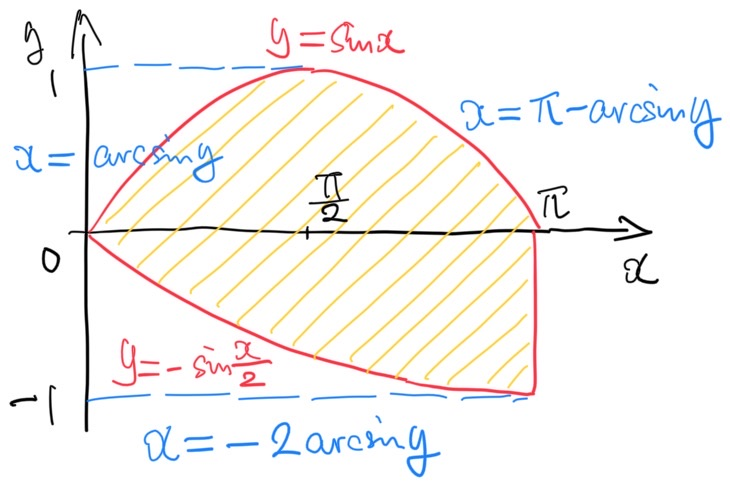
\includegraphics[width=0.45\textwidth]{./images/ch10/10.2.1.3.jpg}
% 		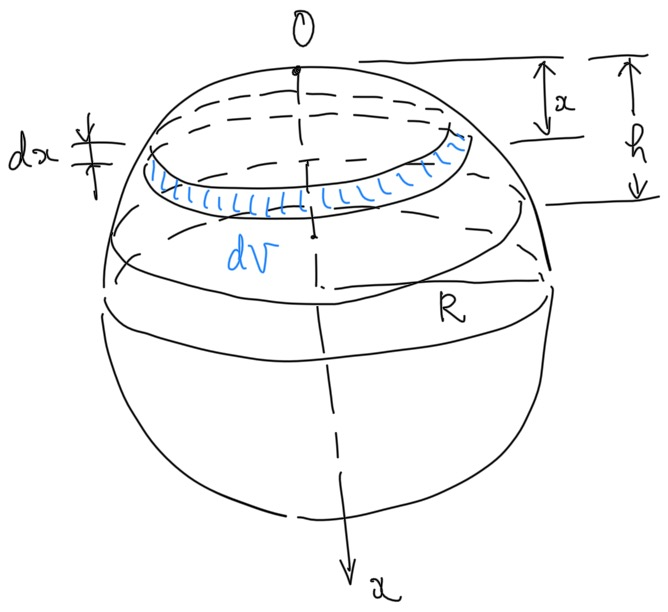
\includegraphics[width=6cm]{./images/ch6/topSp.jpg}
	\end{center}
	\small 解:\it
	如图,
	$$\mbox{原式}=\left(\dint_{-1}^0\dint_{-2\arcsin y}^{\pi}
	+\dint_0^1\dint_{\arcsin y}^{\pi-\arcsin y}\right)
	f(x,y)\d x\d y$$
\end{frame}

\begin{frame}
	\linespread{1.5}
	\ba{(4)$\dint_0^1\dint_{1+\sqrt{1-x^2}}^{\sqrt{4-x^2}}f(x,y)\d y\d x
	+\dint_1^{\sqrt3}\dint_1^{\sqrt{4-x^2}}f(x,y)\d y\d x$}

	\bigskip
	
	\begin{columns}
		\begin{column}{.45\textwidth}
			\begin{center}
				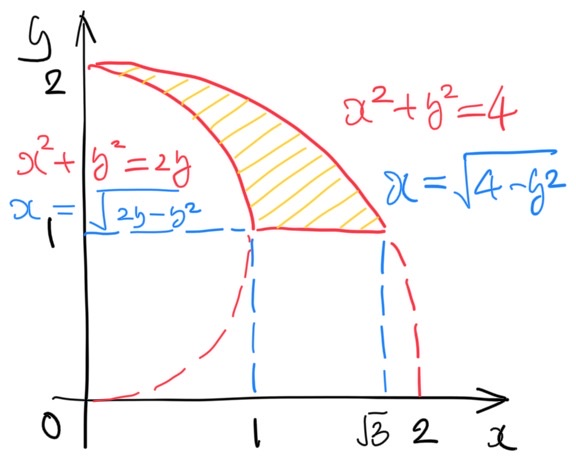
\includegraphics[width=\textwidth]{./images/ch10/10.2.1.4.jpg}
		% 		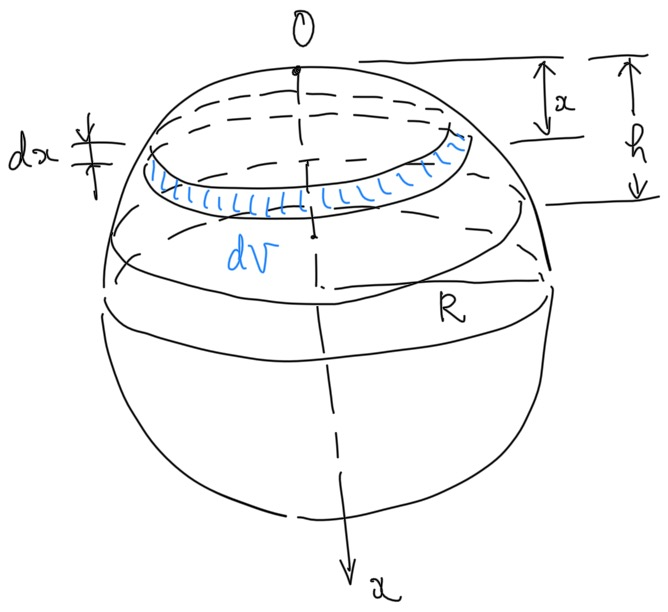
\includegraphics[width=6cm]{./images/ch6/topSp.jpg}
			\end{center}
		\end{column}
		\begin{column}{.55\textwidth}
			\small 解:\it
			如图,
			$$\mbox{原式}=\dint_1^2\dint_{\sqrt{2y-y^2}}^{\sqrt{4-y^2}}
			f(x,y)\d x\d y$$
		\end{column}
	\end{columns}
\end{frame}

\begin{frame}
	\linespread{1.5}
	\ba{2.计算积分
	$\dint_0^e\dint_1^2\df{\ln x}{e^x}\d x\d y
	+\dint_e^{e^2}\dint_{\ln y}^2\df{\ln x}{e^x}\d x\d y.$}

	\bigskip
	
	\begin{columns}
		\begin{column}{.45\textwidth}
			\begin{center}
				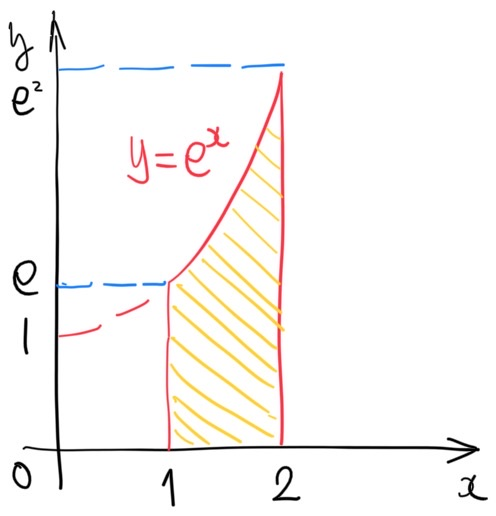
\includegraphics[width=0.9\textwidth]{./images/ch10/10.2.2.jpg}
		% 		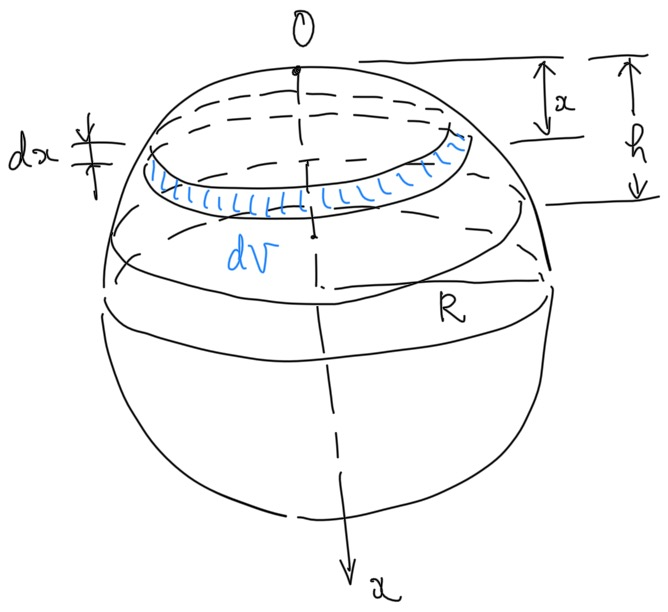
\includegraphics[width=6cm]{./images/ch6/topSp.jpg}
			\end{center}
		\end{column}
		\begin{column}{.55\textwidth}
			\small 解:\it
			如图,
			\begin{align*}
			\mbox{原式}
			&=\dint_1^2\dint_0^{e^x}\df{\ln x}{e^x}\d y\d x
			=\dint_1^2\ln x\d x\\
			&=\dint_0^{\ln 2}u\d e^u
			=\left.ue^u\right|_0^{\ln 2}-\dint_0^{\ln 2}e^u\d u\\
			&=2\ln2-1.
		\end{align*}
		\end{column}
	\end{columns}
\end{frame}

\begin{frame}
	\linespread{1.5}
	\ba{3.求函数$V(t)=\ds\iint_{D_t}[(t-1)y+1]\d\sigma$的最大值,其中
	$D_t:x^2+y^2\leq1,-\df1{t-1}\leq y\leq1$,$2\leq t\leq3$。}
	
	\begin{center}
		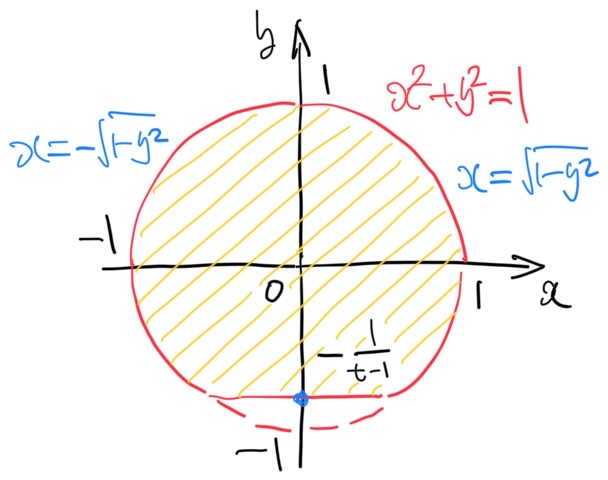
\includegraphics[width=0.5\textwidth]{./images/ch10/10.2.3.jpg}
% 		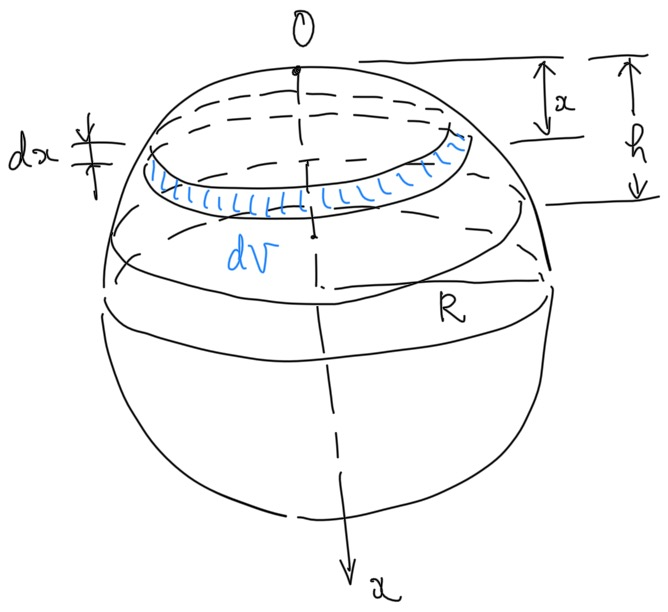
\includegraphics[width=6cm]{./images/ch6/topSp.jpg}
	\end{center}
	
	\small 解:\it 如图
	$D:-\df1{t-1}\leq y\leq 1,\;-\sqrt{1-y^2}\leq x\leq \sqrt{1-y^2}.$
\end{frame}

\begin{frame}
	\linespread{1.5}
	\small\it 
	\begin{align*}
		V(t)&=\dint_{-\frac1{t-1}}^1\dint_{-\sqrt{1-y^2}}^{\sqrt{1-y^2}}
		[(t-1)y+1]\d x\d y\\
		&=2\dint_{-\frac1{t-1}}^1[(t-1)y+1]\sqrt{1-y^2}\d y
	\end{align*}
	从而
	$$V'(t)=2\dint_{-\frac1{t-1}}^1y\sqrt{1-y^2}\d y.$$
	
	\ba{请认真复习一下变限积分求导的有关方法!}
\end{frame}

\begin{frame}
	\linespread{1.5}
	\small\it 
	注意到$2\leq t\leq 3$时,$-1\leq-\df1{t-1}\leq-\df12$。
	由对称性可知
	$\dint_{-\frac1{t-1}}^{\frac1{t-1}}y\sqrt{1-y^2}\d y=0$,
	又$t\in\left[\frac1{t-1},1\right]$时,$y\sqrt{1-y^2}>0$,故
	\begin{align*}
		V'(t)&=2\left(\dint_{-\frac1{t-1}}^{\frac1{t-1}}+
		\dint_{\frac1{t-1}}^1\right)y\sqrt{1-y^2}\d y
		=2\dint_{\frac1{t-1}}^1y\sqrt{1-y^2}\d y>0.
	\end{align*}
	从而可知$t=3$时$V(t)$取最大值,此时
	\begin{align*}
		V(3)&=2\dint_{-\frac12}^1(2y+1)\sqrt{1-y^2}\d y
		=\df{3\sqrt3}4+\df{2\pi}3.
	\end{align*}
	\fin
\end{frame}


\begin{frame}
	\linespread{1.5}
	\ba{4.计算下列二重积分:
	
	(1)$\ds\iint_Dxye^{xy^2}\d\sigma,\,D=\{0\leq x\leq 1,0\leq y\leq 1\}$}

	\bigskip
	
	\small 解:\it
	\begin{align*}
		\mbox{原式}&=\dint_0^1\dint_0^1xye^{xy^2}\d y\d x
		=\df12\dint_0^1\left.e^{xy^2}\right|_{y=0}^{y=1}\d x
		=\df12\dint_0^1(e^x-1)\d x=\df12(e-2).
	\end{align*} \fin
\end{frame}

\begin{frame}
	\linespread{1.5}
	\ba{(2)$\ds\iint_D\df 1{x+y}\d\sigma,\,D=\{0\leq x\leq 1,1\leq x+y\leq2\}$}

	\bigskip
	
	\begin{columns}
		\begin{column}{.45\textwidth}
			\begin{center}
				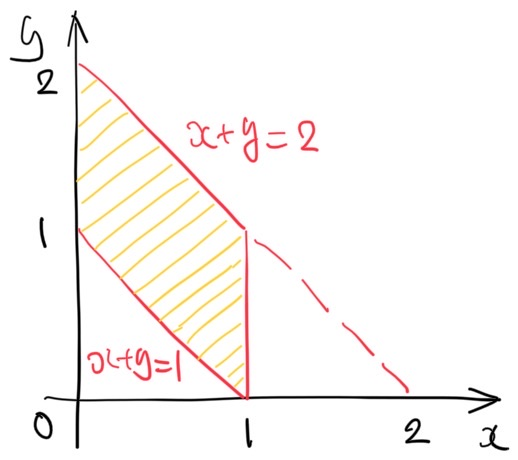
\includegraphics[width=0.9\textwidth]{./images/ch10/10.2.4.2.jpg}
		% 		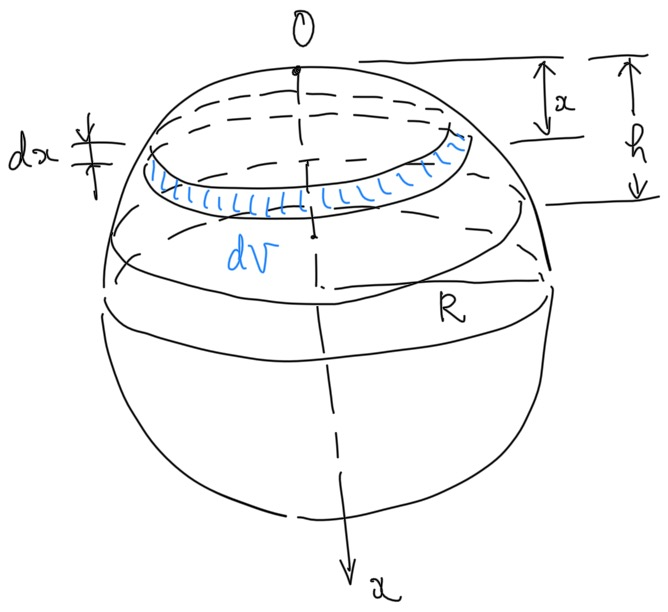
\includegraphics[width=6cm]{./images/ch6/topSp.jpg}
			\end{center}
		\end{column}
		\begin{column}{.55\textwidth}
			\small 解:\it
			区域$D$可表示为
			$$D:0\leq x\leq 1,\; 1-x\leq y\leq 2-x,$$
			于是
			\begin{align*}
				\mbox{原式}&=\dint_0^1\dint_{1-x}^{2-x}\df1{x+y}\d y\d x\\
				&=\dint_0^1\left.\ln|x+y|\right|_{y=1-x}^{y=2-x}\d x\\
				&=\dint_0^1\ln 2\d x=\ln2.
			\end{align*}
		\end{column}
	\end{columns}
\end{frame}

\begin{frame}
	\linespread{1.5}
	\ba{(3)$\ds\iint_D|x^2+y^2-4|\d\sigma,\,D=\{x^2+y^2\leq 9\}$ }

	\bigskip
	
	\begin{columns}
		\begin{column}{.45\textwidth}
			\begin{center}
				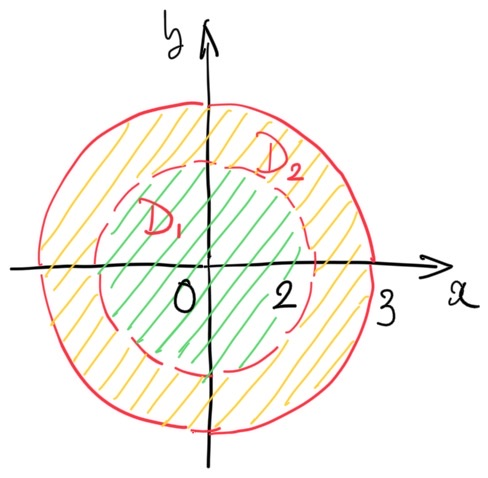
\includegraphics[width=0.9\textwidth]{./images/ch10/10.2.4.3.jpg}
		% 		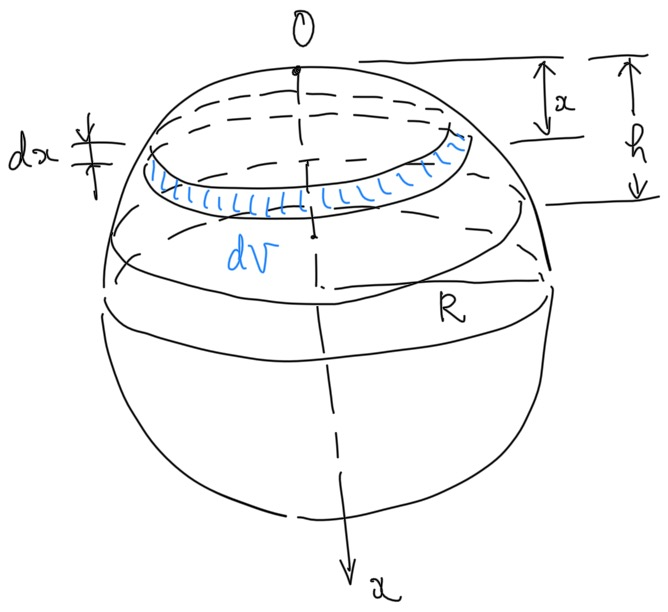
\includegraphics[width=6cm]{./images/ch6/topSp.jpg}
			\end{center}
		\end{column}
		\begin{column}{.55\textwidth}
			\small 解:\it
			\begin{align*}
				\mbox{原式}&=\left(\iint_{D_1}+\iint_{D_2}\right)|x^2+y^2-4|\d\sigma\\
				&=\iint_{D_1}(4-x^2-y^2)\d\sigma)+\iint_{D_2}(x^2+y^2-4)\d\sigma\\
				&=\dint_0^{2\pi}\dint_0^2(4-\rho^2)\rho\d\rho\d\theta\\
				&\;\;+\dint_0^{2\pi}\dint_2^3(\rho^2-4)\rho\d\rho\d\theta\\
				&=\df{41}2\pi
			\end{align*}
		\end{column}
	\end{columns}
\end{frame}

\begin{frame}
	\linespread{1.5}
	\ba{(4)$\ds\iint_D\ln(x^2+y^2)^{\frac12}\d\sigma,\,
	D=\{1\leq x^2+y^2\leq e^2\}$}

	\bigskip
	
	\small 解:\it
	令$x=\rho\cos\theta,y=\rho\sin\theta$,则
	$$D:1\leq\rho\leq e,0\leq\theta\leq2\pi,$$
	从而
	\begin{align*}
		\mbox{原式}&=\dint_0^{2\pi}\dint_1^e\rho\ln\rho\d\rho\d\theta
		=\df{1+e^2}2\pi
	\end{align*}
	\fin
\end{frame}

\begin{frame}
	\linespread{1.5}
	\ba{5.计算二重积分$\ds\iint_D(x^2+y^2)\d\sigma$,其中$D$由$y=-x,
	x=\sqrt{4-y^2}$和$y=\sqrt{2x-x^2}$所围成。}
	
	\begin{columns}
		\begin{column}{.4\textwidth}
			\begin{center}
				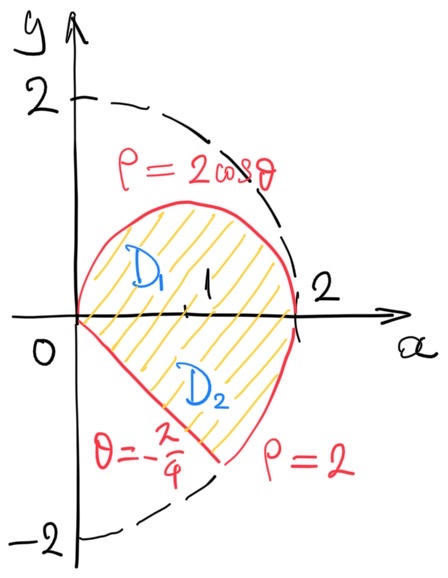
\includegraphics[width=0.9\textwidth]{./images/ch10/10.2.5-1.jpg}
		% 		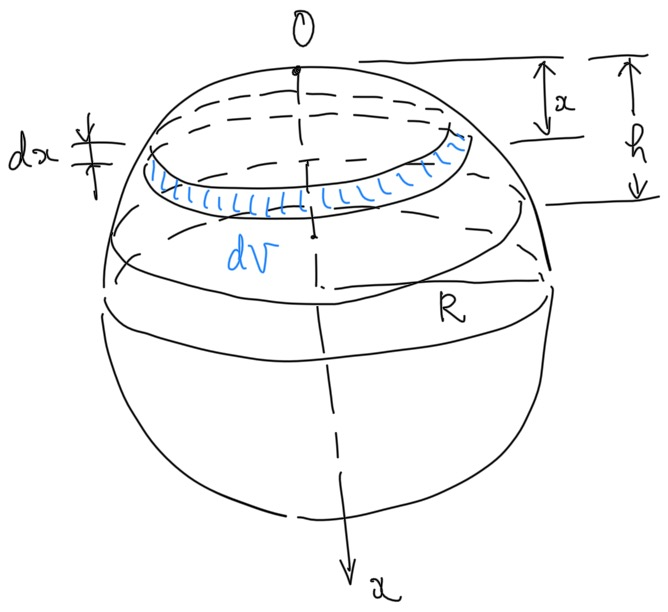
\includegraphics[width=6cm]{./images/ch6/topSp.jpg}
			\end{center}
		\end{column}
		\begin{column}{.6\textwidth}
			\small 要点:\it
			$$D_1:0\leq\theta\leq\df{\pi}2,0\leq\rho\leq2\cos\theta,$$
			$$D_2:-\df{\pi}4\leq\theta\leq0,0\leq\rho\leq2,$$
			\begin{align*}
				\mbox{原式}&=\left(\iint_{D_1}+\iint_{D_2}\right)(x^2+y^2)\d\sigma\\
				&=\dint_0^{\frac{\pi}2}\dint_0^{2\cos\theta}\rho^3\d\rho\d\theta
				+\dint_{-\frac{\pi}4}^0\dint_0^2\rho^3\d\rho\d\theta\\
				&=\df74\pi.
			\end{align*}
		\end{column}
	\end{columns}
\end{frame}

\begin{frame}
	\linespread{1.5}
	\ba{另解:}
	\begin{center}
		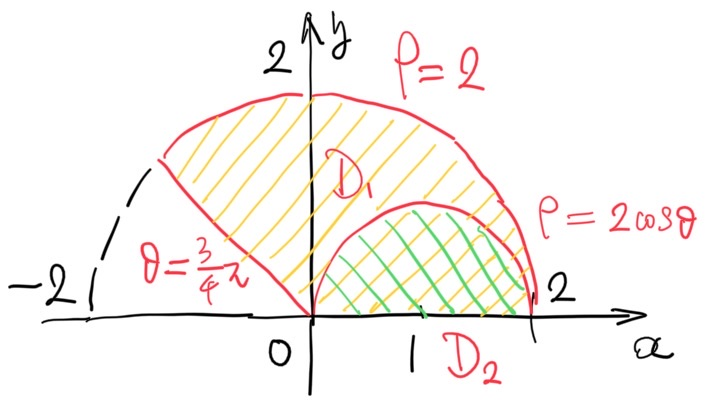
\includegraphics[width=0.6\textwidth]{./images/ch10/10.2.5-2.jpg}
% 		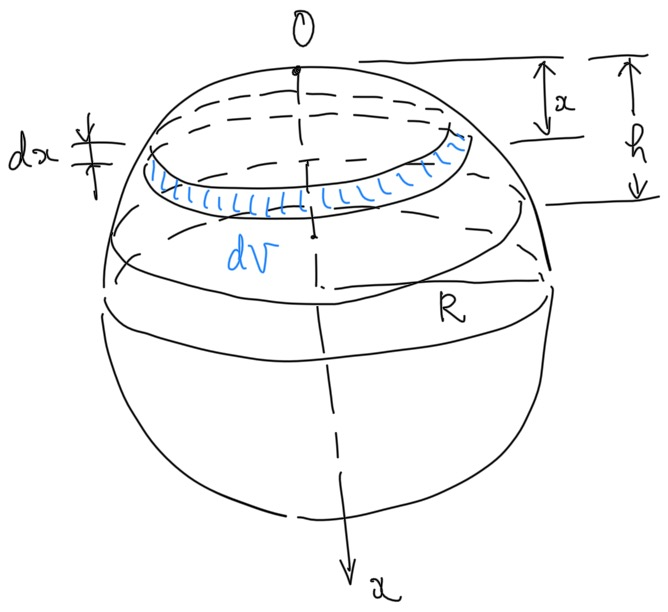
\includegraphics[width=6cm]{./images/ch6/topSp.jpg}
	\end{center}
	\small 要点:\it
	$$D_1:0\leq\theta\leq\df{3\pi}4,0\leq\rho\leq 2,
	D_2:0\leq\theta\leq\df{\pi}2,0\leq\rho\leq 2\cos\theta,$$
	最终积分结果为$\df94\pi$。
\end{frame}

\begin{frame}
	\linespread{1.5}
	\ba{6.已知$f(x)$在原点附近连续,$D:x^2+y^2\leq t^2$,计算极限
	$\lim\limits_{t\to0^+}\df1{\pi t^2}\iint_Df(\sqrt{x^2+y^2})\d\sigma$。}
	\pause

	\bigskip
	\small 解:\it
	令$x=\rho\cos\theta,y=\rho\sin\theta$,区域$D$可表示为
	$$D:0\leq\theta\leq2\pi,0\leq\rho\leq t,$$
	于是
	\begin{align*}
		\mbox{原式}&=\lim\limits_{t\to0^+}\df1{\pi t^2}
		\dint_0^t\dint_0^{2\pi}f(\rho)\rho\d\theta\d\rho
		=\lim\limits_{t\to0^+}\df{2\pi f(t)t}{2\pi t}=f(0).
	\end{align*}
	\fin
\end{frame}

% \begin{frame}{出现的问题}
% 	\linespread{1.5}
% 	  \begin{itemize}%[<+-|alert@+>]
% 	    \item 作业进度慢!
% 	    \item 概念问题
% 	    \begin{itemize}
% 	      \item \b\it 幂级数展开不熟练
% 	      \item \b\it Maclaurin级数和关于$(x-x_0)$的幂级数分不清
% 	    \end{itemize}
% 	    \item 过程不规范或不完整
% 	    \begin{itemize}
% 	      \item \b\it 求收敛域要单独讨论端点的敛散性
% 	      \item \b\it 相同幂次的项要合并,并按幂次从小到大排列
% 	      \item \b\it 书写潦草随意\pause
% 	    \end{itemize}
% 	    \item \ba{雷同!!!}
% 	  \end{itemize}
% \end{frame}

% \begin{frame}
% 	\linespread{1.5}
% 	\ba{3.设$D$是由曲线$y=\sin x+1$与三条直线$x=0,x=\pi,y=0$
% 	所围成的曲边梯形,求$D$绕$x$轴旋转一周所围成的旋转体的体积。
% 	}
% 	\pause
% 	
% % 	\bigskip
% 	
% 	\begin{columns}
% 		\begin{column}{.5\textwidth}
% 			\begin{center}
% 				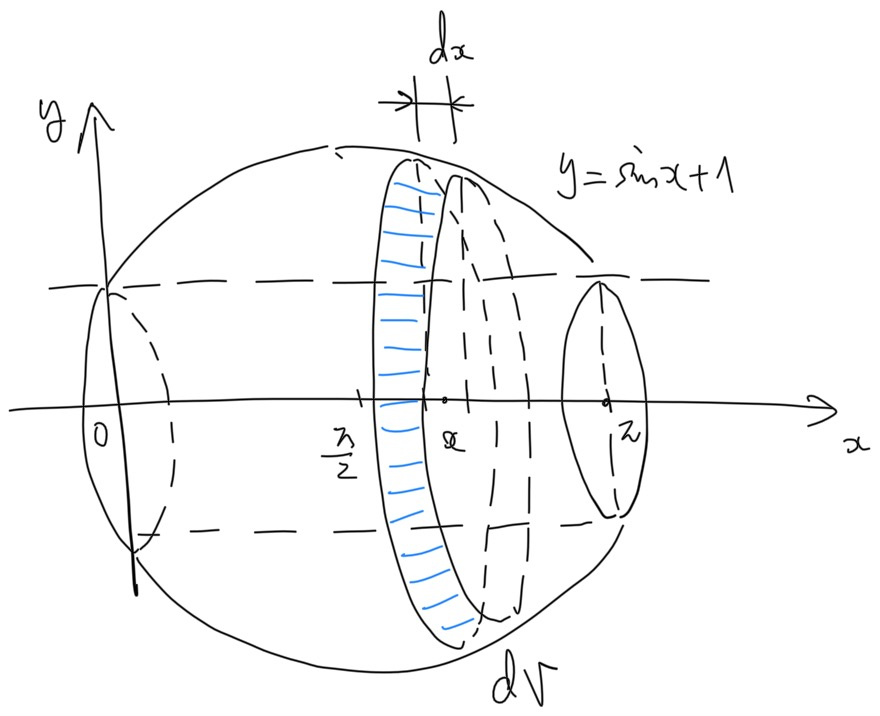
\includegraphics[width=.9\textwidth]{./images/ch6/sinx1cs.jpg}
% 		% 		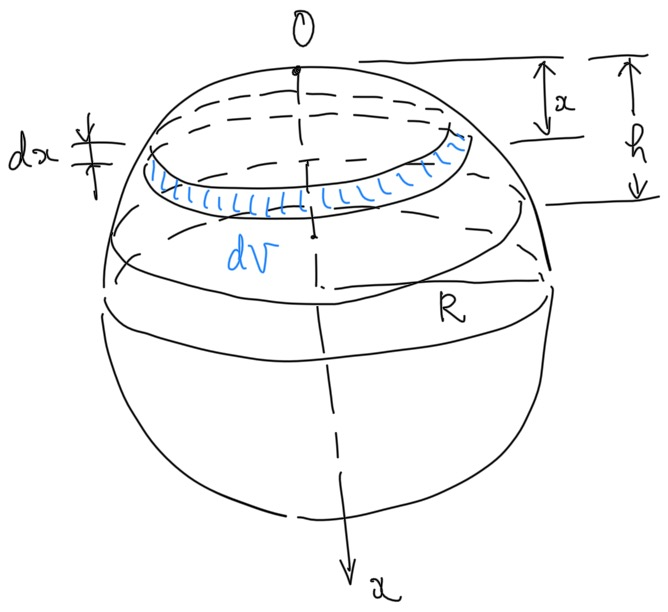
\includegraphics[width=6cm]{./images/ch6/topSp.jpg}
% 			\end{center}		
% 		\end{column}
% 		\begin{column}{.5\textwidth}
% 			\small 解:\it
% 			如图,体积微元$\d V=\pi y^2\d x$,	故所求体积
% 			$$
% 				V=\dint_0^{\pi}\pi(\sin x+1)^2\d x=\df32\pi^2.
% 			$$
% 		\end{column}
% 	\end{columns}
% \end{frame}